\chapter{计数}
\label{chap:combinatorics}
\label{chap:counting}

从四门课中任选一些，共有多少种选法？从四名学生中选出组长和记录员，又有多少种安排？
对象稍多时，逐一列举既费力又容易重复或遗漏。本章研究怎样不逐一列举而算出有限集合的元素个数。

计数前先要确定什么算一个结果。从四个对象中依次取两个，$(1,3)$与$(3,1)$是不同的有序记录；
若只记录选中了哪些对象，它们都是子集$\{1,3\}$。记录方式不同，结果数也不同。
元素个数借助第~\ref{chap:sets-relations-maps}章的双射来说明：有限集合$A$有$n$个元素，是说存在双射$\{1,\ldots,n\}\to A$，
即能把$A$的元素恰好编号为$1,\ldots,n$；空集对应$n=0$。$A$的元素个数记为$|A|$。

本章先推出加法规则和乘法规则，再算出排列、组合、子集与划分的数量，最后用容斥原理处理类别重叠，用递推处理可化为更小同类问题的情形。
以下记$V=\{1,\ldots,n\}$，其中$n\geq0$。

\section{分类和分步计数}
\label{sec:comb-families-counting}
\label{sec:comb-finite-counting}
\label{sec:comb-decomposition-counting}
\label{sec:comb-classification-products}
\label{sec:comb-classification-counting}

本节的三条规则对应三种做法：把要数的集合换成更容易数的集合，把结果分成互不重叠的几类，把每个结果拆成依次进行的几步选择。

\paragraph{双射与计数}
数出有限集合$A$有$n$个元素，就是给出编号双射$g:\{1,\ldots,n\}\to A$。若另有双射$f:A\to B$，
则$f\circ g$把$B$的元素也恰好编号为$1,\ldots,n$。所以两个有限集合之间存在双射时，元素个数相同；
因此，可以通过计算一个较容易计数、且与原集合一一对应的集合的大小，得到原集合的元素个数。

同一个集合也不会数出两个不同的个数：若$h:\{1,\ldots,m\}\to\{1,\ldots,n\}$是双射，则$m=n$。
对$n$归纳：$n=0$时源集也只能为空，即$m=0$；$n\geq1$时$m\geq1$，设$h(j)=n$，交换$h$在$j$与$m$处的取值，
使$m$对应$n$，再把交换后的映射限制到$\{1,\ldots,m-1\}$，得到到$\{1,\ldots,n-1\}$的双射，由归纳假设$m-1=n-1$。

\paragraph{加法规则}
若有限集合$A_1,\ldots,A_r$两两不交，则
\[
 \Bigl|\bigcup_{i=1}^r A_i\Bigr|=\sum_{i=1}^r|A_i|,
\]
这称为计数的加法规则。它来自编号的拼接：先给$A_1$的元素编号$1,\ldots,|A_1|$，再接着给$A_2$编号，依此类推；
两两不交保证没有元素被编号两次。使用时要检查各类覆盖全部结果且两两不交；类别重叠的情形留给第~\ref{sec:comb-overlap-counting}节的容斥原理。
由加法规则，若$B\subsetneq A$都是有限集合，则$|A|=|B|+|A\setminus B|>|B|$，即有限集合的真子集元素更少。

加法规则的一个推论是\term{抽屉原理}（pigeonhole principle）：把$m$个对象放进$k$个位置，若每个位置至多一个对象，
按位置分类得$m\leq k$；因此$m>k$时必有某个位置容纳至少两个对象。例如任选$13$人，必有两人同月出生。
换句话说，$m>k$时从$m$元集到$k$元集的映射都不是单射。

\paragraph{乘法规则}
\phantomsection
\label{sec:comb-stepwise-counting}
对有限集合$A_1,\ldots,A_r$，
\[
 |A_1\times\cdots\times A_r|=\prod_{i=1}^r|A_i|,
\]
这称为计数的乘法规则。$r=2$时，按第一个位置的取值把$A_1\times A_2$分成$|A_1|$类，
第$a$类$\{a\}\times A_2$与$A_2$之间有双射$(a,b)\mapsto b$，由加法规则得$|A_1|\cdot|A_2|$；一般的$r$对位置个数归纳。
例如第一位取$a,b$之一、第二位取$1,2,3$之一，共有$2\times3=6$个结果，逐一列出即$(a,1),(a,2),(a,3),(b,1),(b,2),(b,3)$；
长度为$n$的零一记录组成$\{0,1\}^n$，共$2^n$条。

分步选择中，后一步的选项常依赖前一步，例如先选组长、再从其余人中选记录员。
只要第$i$步在每种已有记录之后都恰有$n_i$个选项，完整记录数仍是$\prod_in_i$：按第一步分成$n_1$类，
每类由归纳假设都有$\prod_{i\geq2}n_i$个记录，再用加法规则。要求的是选项的个数固定，选项的内容可以变化。
若个数也随前一步改变，就先分类再相加。例如从四门课中选一门主修，主修课程$1$时只能从课程$2,3$中选辅修，
否则可从其余三门中选，完整记录数是$1\times2+3\times3=11$。

\section{排列与组合}
\label{sec:comb-permutation-combination-counts}
\label{sec:comb-subset-partition-counts}

选取若干对象时，可以记录它们所在的位置，也可以只记录选中了谁。先按位置计数，再把只是位置不同的记录归为一类，
就能联系这两类问题；不限选取个数或二分对象时，则可以借助零一记录。

\paragraph{排列数}
设$0\leq k\leq n$。从$n$个不同对象中取出$k$个依次放在$k$个位置上且不重复，所得有序$k$元组称为排列，个数记为$P(n,k)$。
各位置依次有$n,n-1,\ldots,n-k+1$种选择，由乘法规则
\[
 P(n,k)=\prod_{i=0}^{k-1}(n-i)=n(n-1)\cdots(n-k+1),
\]
$k=0$时为空积$1$，对应唯一的空排列。例如从四人中选组长和记录员有$P(4,2)=12$种安排。
$n(n-1)\cdots1$记作$n!$，称为$n$的\term{阶乘}（factorial），约定$0!=1$，于是$P(n,k)=n!/(n-k)!$。

若允许重复选取，每个位置都有$n$个选项，有序记录数是$n^k$；例如连续两天从三道菜中各选一道，允许重复时有$9$种，不允许时有$6$种。

\paragraph{组合数}
若只记录选中的对象，结果是一个$k$元子集，称为组合，个数记为$\binom nk$，读作“$n$选$k$”。
每个排列确定一个$k$元子集，每个$k$元子集又恰好对应$k!$个排列，所以全部排列按子集分成$\binom nk$类，每类$k!$个，
加法规则给出$P(n,k)=\binom nk k!$，即
\begin{equation}
 \binom nk=\frac{P(n,k)}{k!}=\frac{n!}{k!(n-k)!},\qquad 0\leq k\leq n.
 \label{eq:prelim-binomial-coefficient}
\end{equation}
例如十二种组长—记录员安排中每个二人小组恰好出现两次，所以二人小组有$6$个。

取补集给出$k$元子集与$(n-k)$元子集的双射，所以$\binom nk=\binom n{n-k}$；$\binom n0=\binom nn=1$分别对应空集与全体，
并约定$k<0$或$k>n$时$\binom nk=0$。允许重复的无序选择则不能直接套用组合数。

从$n$种水果中挑$k$个、同种不加区分，结果由各种的个数$(m_1,\ldots,m_n)$决定，$\sum_im_i=k$。
依次写$m_1$个星号、一条竖线、$m_2$个星号……，得到$k$个星号与$n-1$条竖线排成的一行，二者一一对应，
所以结果数是从$n+k-1$个位置中选出星号位置的方法数$\binom{n+k-1}{k}$。例如从三种水果中挑两个，有$\binom42=6$种。

\paragraph{幂集与组合恒等式}
\phantomsection
\label{sec:comb-ordered-unordered}
每个子集$S\subseteq V$对应一条零一记录$(z_1,\ldots,z_n)$，$z_i=1$当且仅当$i\in S$；这是$\mathcal P(V)$到$\{0,1\}^n$的双射，所以
\begin{equation}
 |\mathcal P(V)|=2^n.
 \label{eq:comb-power-set-count}
\end{equation}
另一方面，按大小把子集分成$0,1,\ldots,n$元子集，加法规则给出子集总数$\sum_k\binom nk$。对同一集合的这两种计数称为双重计数，它给出
\[
 \sum_{k=0}^n\binom nk=2^n.
\]

交错和$\sum_k(-1)^k\binom nk$等于偶数大小子集数减去奇数大小子集数。当$n\geq1$时，固定元素$n$，
对每个子集作“含$n$则删去、不含则加入”的改动；它是$\mathcal P(V)$到自身的双射，并把子集大小改变$1$，
因而把偶数大小的子集一一配对到奇数大小的子集，所以
\begin{equation}
 \sum_{k=0}^n(-1)^k\binom nk=0,\qquad n\geq1.
 \label{eq:comb-alternating-subset-count}
\end{equation}
$n=0$时交错和为$1$。下一节的容斥原理就依靠这一抵消。

\paragraph{二分划分}
把$V$的对象分到有名称的两侧，例如“已选”和“未选”，结果$(S,V\setminus S)$由$S$唯一确定，共$2^n$个。

若两侧没有名称，结果是$\{S,V\setminus S\}$；$n\geq1$时$S\neq V\setminus S$，每个无名称结果恰有两个有名称表示，
所以无名称结果有$2^{n-1}$个。

要求两侧非空时，去掉$(\varnothing,V)$与$(V,\varnothing)$，得到$2^n-2$个有名称结果与$2^{n-1}-1$个无名称结果。

$n=0$时只有$(\varnothing,\varnothing)$，两侧相同，不能用除以$2$的公式。

\section{重叠计数与递推计数}
\label{sec:comb-overlap-counting}
\label{sec:comb-inclusion-mobius}

本节处理加法规则不能直接使用的两种情形：类别重叠时用交集校正重复计数；问题能化为更小的同类问题时建立递推。

\paragraph{容斥原理}
设$A=\{1,2,3,4\}$、$B=\{3,4,5\}$。$|A|+|B|=7$把公共元素$3,4$各数了两次，减去交集得$|A\cup B|=7-2=5$。
一般地，把并集分成$A\setminus B$、$A\cap B$、$B\setminus A$三个不交部分并用加法规则，得到
\[
 |A\cup B|=|A|+|B|-|A\cap B|.
\]
图~\ref{fig:comb-inclusion-exclusion-overlap}显示了被多数一次的公共区域。
\begin{figure}[htbp]
  \centering
  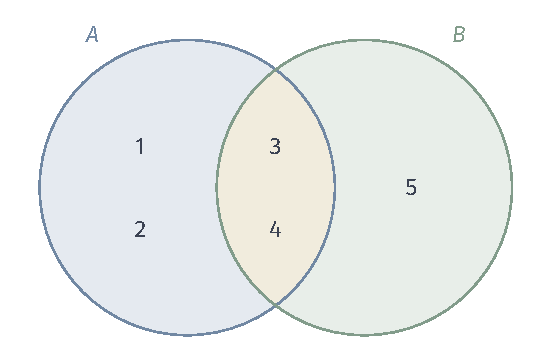
\includegraphics[width=90mm]{figures/00-shared/mathematical-preliminaries-upper/01-mathematical-language-combinatorics-analysis-optimization/tikz/inclusion-exclusion-overlap.pdf}
  \caption{两个有限集合的重叠计数。$A=\{1,2,3,4\}$，$B=\{3,4,5\}$；仅属于$A$的区域放入$1,2$，公共区域放入$3,4$，仅属于$B$的区域放入$5$。把两圈元素个数相加时，公共区域被数两次，减去一次后得到并集中的五个不同元素。}
  \label{fig:comb-inclusion-exclusion-overlap}
\end{figure}

对三个集合逐元素检查：恰属于两个集合的元素先计两次、再减一次；同属三者的元素先计三次、减三次，还需加回一次。所以
\[
 |A\cup B\cup C|=|A|+|B|+|C|-|A\cap B|-|A\cap C|-|B\cap C|+|A\cap B\cap C|.
\]
\term{容斥原理}（inclusion--exclusion principle）把这种交替加减推广到任意有限个集合。
\begin{theorem}[有限容斥原理]
\label{thm:comb-inclusion-exclusion}
设$A_1,\ldots,A_m$是有限集合。则
\begin{equation}
  \Bigl|\bigcup_{i=1}^{m}A_i\Bigr|
  =\sum_{\varnothing\neq I\subseteq\{1,\ldots,m\}}(-1)^{|I|+1}\Bigl|\bigcap_{i\in I}A_i\Bigr|.
  \label{eq:comb-inclusion-exclusion}
\end{equation}
\end{theorem}
\begin{proof}
左侧每个并集元素恰计一次。右侧按元素合并，只需检查每个元素$x$的总系数。
设$x$恰属于$r$个集合，其下标组成$J$；$x$属于$\bigcap_{i\in I}A_i$当且仅当$I\subseteq J$。
$r=0$时$x$不在并集中，两侧都不计入。$r\geq1$时，大小为$k$的$I\subseteq J$有$\binom rk$个，所以$x$的总系数为
\[
 \sum_{k=1}^r(-1)^{k+1}\binom rk=-\Bigl(\sum_{k=0}^r(-1)^k\binom rk-1\Bigr)=1,
\]
最后一步用式~\eqref{eq:comb-alternating-subset-count}。所以两侧相等。
\end{proof}

\paragraph{补集计数}
有多条限制时，可以先数违反限制的结果，再从总数中减去。四门课的选法记作$\bm z=(z_1,z_2,z_3,z_4)\in\{0,1\}^4$，$z_i=1$表示选第$i$门。
规则是：课程$1,2$恰选一门；选课程$3$就必须选课程$1$；选课程$4$就必须在课程$2,3$中至少选一门。违反各条规则的选法分别组成
\[
 \begin{aligned}
 A_1&=\{\bm z:z_1=z_2\},\\
 A_2&=\{\bm z:z_3=1,\ z_1=0\},\\
 A_3&=\{\bm z:z_4=1,\ z_2=z_3=0\}.
 \end{aligned}
\]
由De Morgan律，合法选法组成$(A_1\cup A_2\cup A_3)^{\mathrm c}$，个数为$16-|A_1\cup A_2\cup A_3|$。
用乘法规则读出$|A_1|=8$、$|A_2|=4$、$|A_3|=2$；$A_1\cap A_2$要求$z_1=z_2=0$、$z_3=1$，有$2$个元素；
$A_1\cap A_3$只含$(0,0,0,1)$；$A_2\cap A_3$要求$z_3$既为$1$又为$0$，是空集。
由容斥原理，违规选法有$8+4+2-2-1-0+0=11$种，合法选法为$5$种，对应的课程集合族是
\begin{equation}
 \mathcal C_0=\bigl\{\{1\},\{1,3\},\{1,3,4\},\{2\},\{2,4\}\bigr\}.
 \label{eq:comb-running-feasible-family}
\end{equation}
直接分支计数也得到同样的五种：$z_1=1$时$z_3$任取、$z_4=1$须$z_3=1$，共三种；$z_2=1$时$z_3=0$、$z_4$任取，共两种。

\paragraph{递推计数}
固定元素$n$，把$V$的$k$元子集分成不含$n$与含$n$两类，分别有$\binom{n-1}k$与$\binom{n-1}{k-1}$个，所以
\[
 \binom nk=\binom{n-1}k+\binom{n-1}{k-1},\qquad n\geq1,
\]
称为Pascal恒等式。把它当作递推：令$a_{0,0}=1$，$0\leq k\leq n$以外的$a_{n,k}=0$，并对$n\geq1$规定
\begin{equation}
 a_{n,k}=a_{n-1,k}+a_{n-1,k-1}.
 \label{eq:comb-binomial-recurrence}
\end{equation}
逐行得到$(1)$、$(1,1)$、$(1,2,1)$、$(1,3,3,1)$、$(1,4,6,4,1)$；越界值取零使两端也适用同一规则。
对$n$归纳，并用Pascal恒等式与越界约定，可知$a_{n,k}=\binom nk$。图~\ref{fig:vol1-add-pascal-recurrence}标出了$\binom42=3+3$的来源。
\begin{figure}[!htb]
  \centering
  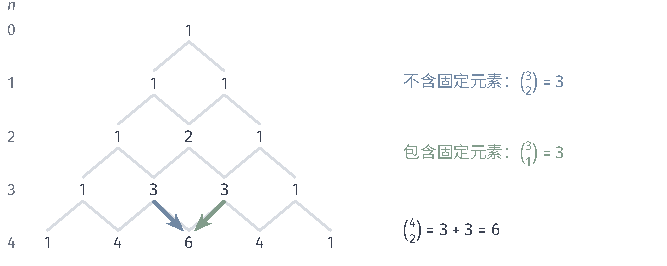
\includegraphics[width=112mm]{figures/00-shared/mathematical-preliminaries-upper/00-shared/tikz/mathematical-language-combinatorics-analysis-optimization-comprehension-additions/pascal-recurrence.pdf}
  \caption{组合数的逐行递推。第$n$行列出$\binom n0,\ldots,\binom nn$；箭头突出$\binom42=\binom32+\binom31=3+3$。两种分类分别从其余三个元素选两个，或先保留固定元素再从其余三个中选一个。网格位置表示递推依赖，不表示子集包含关系。}
  \label{fig:vol1-add-pascal-recurrence}
\end{figure}

一般地，按固定元素、规模或最后一步分类，使每类成为更小的同类问题，就能建立递推。
例如长度为$n$、不含相邻两个$1$的零一记录个数$f_n$：按最后一位分类，末位为$0$时前$n-1$位任意合格，
末位为$1$时倒数第二位须为$0$、前$n-2$位任意合格，所以$f_n=f_{n-1}+f_{n-2}$（$n\geq2$），$f_0=1$、$f_1=2$。
递推式须与初值、适用范围一起写明。由各子集的累计值恢复其自身贡献的Möbius反演，放在图部分第~\ref{sec:comb-cumulative-inversion}节。

\section{本章小结}
\label{sec:comb-summary}

计数先确定什么算一个结果：是否区分次序、是否允许重复、各部分是否有名称。双射把难数的集合换成好数的集合；
互斥类别用加法，抽屉原理是其推论；各步选项数固定时用乘法，否则先分类再相加。
每个结果被记录同样多次时，记录数等于结果数乘以重复次数，排列数、组合数与二分划分的公式都由此得到；
允许重复的无序选择要先换成星号与竖线的记录。双重计数给出组合数之和，增删固定元素的配对给出交错和。
类别重叠时，容斥原理使每个元素恰计一次，补集计数借助De Morgan律把“满足全部限制”改写为“不违反任何一条”；
按固定元素、规模或最后一步分类可以建立递推。

这些方法依赖有限集合能被编号到某个$n$为止。对数不到最后一个元素的无限集合，
仍可以问两个集合的元素能否一一配对；第~\ref{chap:cardinality}章用双射和单射回答这一问题。
